%%% Local Variables:
%%% mode: latex
%%% TeX-master: t
%%% End:

\documentclass[aspectratio=169, compress]{beamer}

% Packages
\usepackage[utf8]{inputenc}
\usepackage{graphicx}
\usepackage{epstopdf}
\usepackage{multimedia}
% Tables
\usepackage{csvsimple}
\usepackage{booktabs}
\usepackage{longtable}
\usepackage{siunitx}
\usepackage{array}
\usepackage{multirow}
\usepackage{natbib}
\usepackage{appendixnumberbeamer}

%Theme
\usetheme{Singapore}
% Disable miniframes
\makeatletter
\let\beamer@writeslidentry@miniframeson=\beamer@writeslidentry%
\def\beamer@writeslidentry@miniframesoff{%
  \expandafter\beamer@ifempty\expandafter{\beamer@framestartpage}{}% does not happen normally
  {%else
    % removed \addtocontents commands
    \clearpage\beamer@notesactions%
  }
}
\newcommand*{\miniframeson}{\let\beamer@writeslidentry=\beamer@writeslidentry@miniframeson}
\newcommand*{\miniframesoff}{\let\beamer@writeslidentry=\beamer@writeslidentry@miniframesoff}
\makeatother

% Auto toc
% \AtBeginSection[]
% {
%   \miniframesoff
%   \begin{frame}
%     \tableofcontents[currentsection]
%   \end{frame}
%   \miniframeson
% }

% \AtBeginSubsection[]
% {
%   \miniframesoff
%   \begin{frame}
%     \tableofcontents[currentsection,currentsubsection]
%   \end{frame}
%   \miniframeson
% }

% figures
\hypersetup{pdfpagemode=FullScreen} % Start in fullscreen
%
\title{Thermodynamic properties of amino acid adsorption over graphene}
\author{Mateo Barría Urenda \\ \vspace{0.1cm} Doctorado en Ciencias
  mención Biofísica y Biología Computacional \\ \vfill 2021}
\date{}

\subtitle{}

\newcommand{\myround}{\tablenum[round-precision=1, round-mode=places,
   table-format=2.1]}

\begin{document}

\begin{frame}[plain]
  \vspace{0.3cm}
  
\includegraphics[height = 1.5cm]{logos/logoDBBC-transp.png}
  \hfill
  
\includegraphics[height = 1.5cm]{logos/Logo-CINV.png}
  \vspace{0.3cm}
  \maketitle
\end{frame}


\begin{frame}{Studies on adsorption processes on graphene}
  \begin{columns}
    \begin{column}{.4\textwidth}
      \centering
      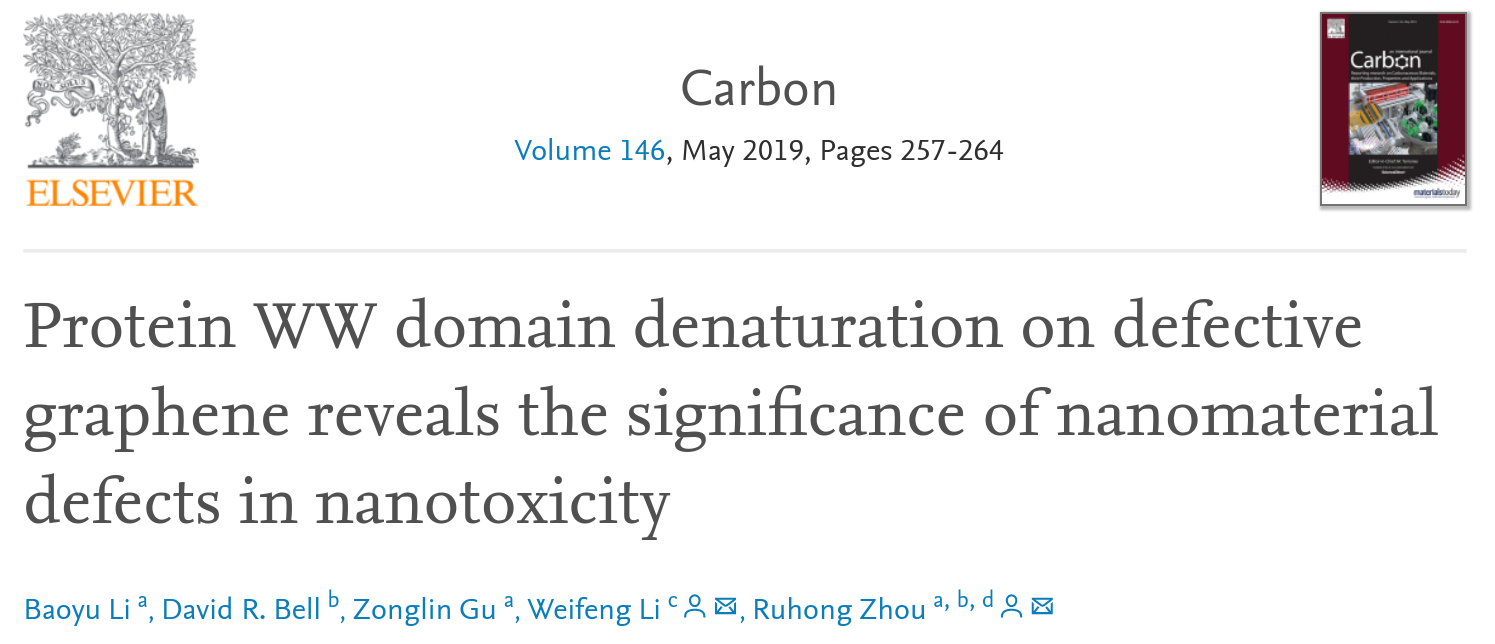
\includegraphics[width=\textwidth]{figures/Adsorption_1} \\
      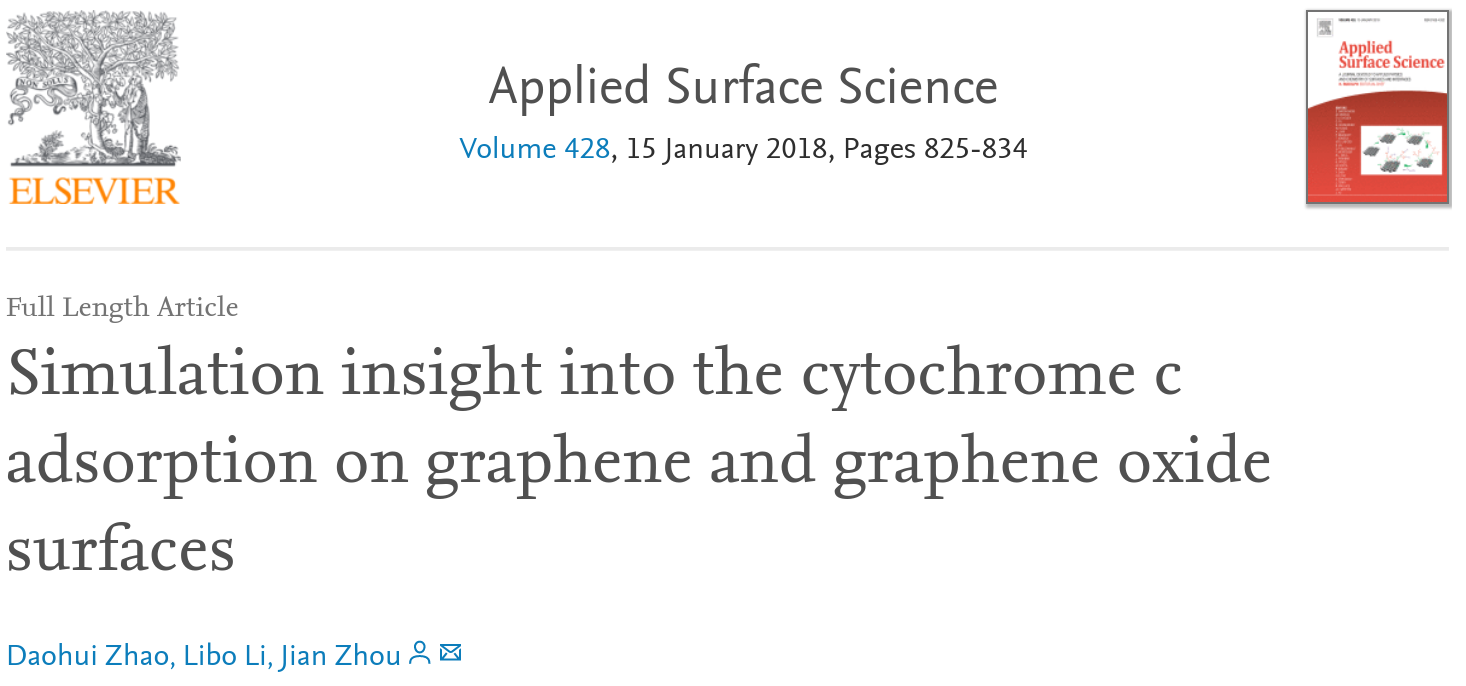
\includegraphics[width=\textwidth]{figures/Adsorption_2}
    \end{column}
    \begin{column}{.6\textwidth}
      \centering
      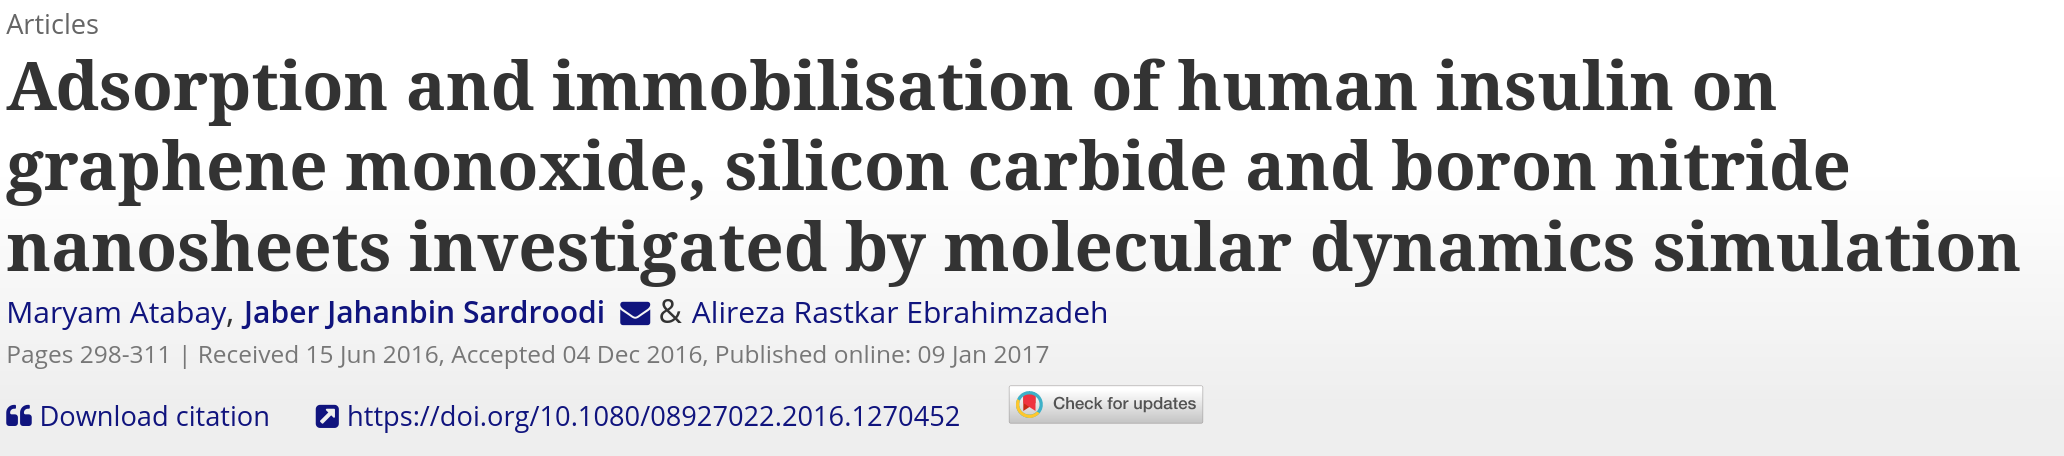
\includegraphics[width=\textwidth]{figures/Adsorption_3}
      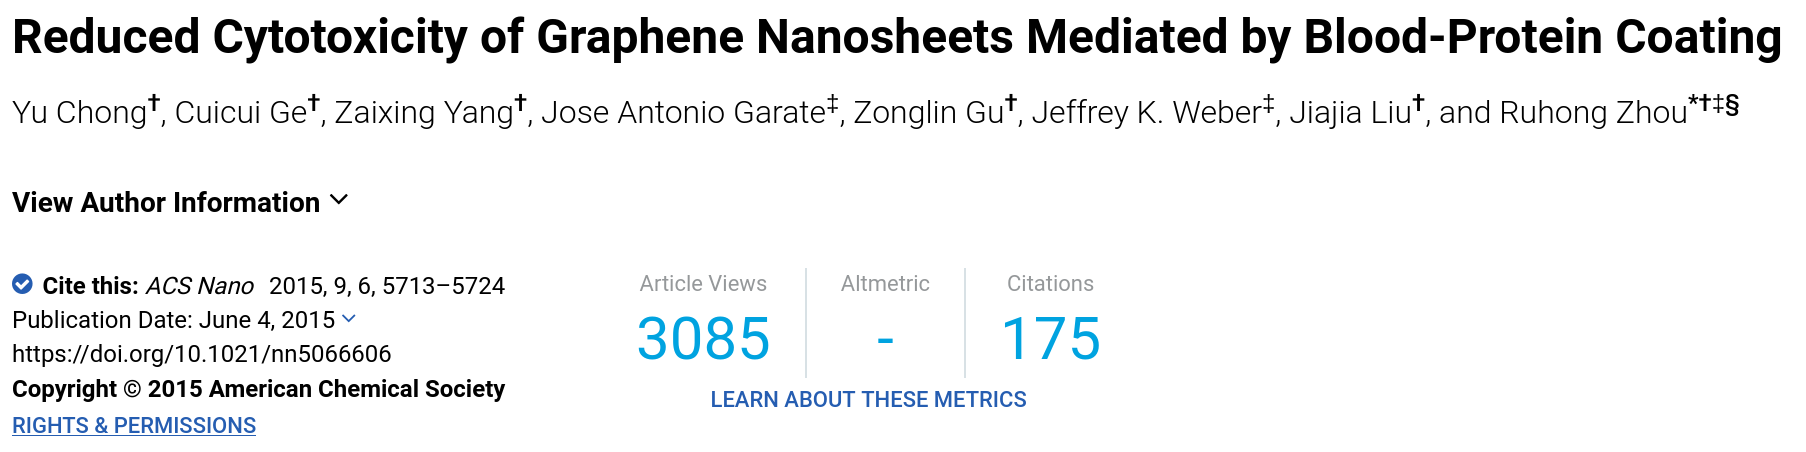
\includegraphics[width=\textwidth]{figures/Adsorption_4}
    \end{column}
  \end{columns}
\end{frame}

\begin{frame}{Graphene can wreak havoc in cell membranes}
  \centering
      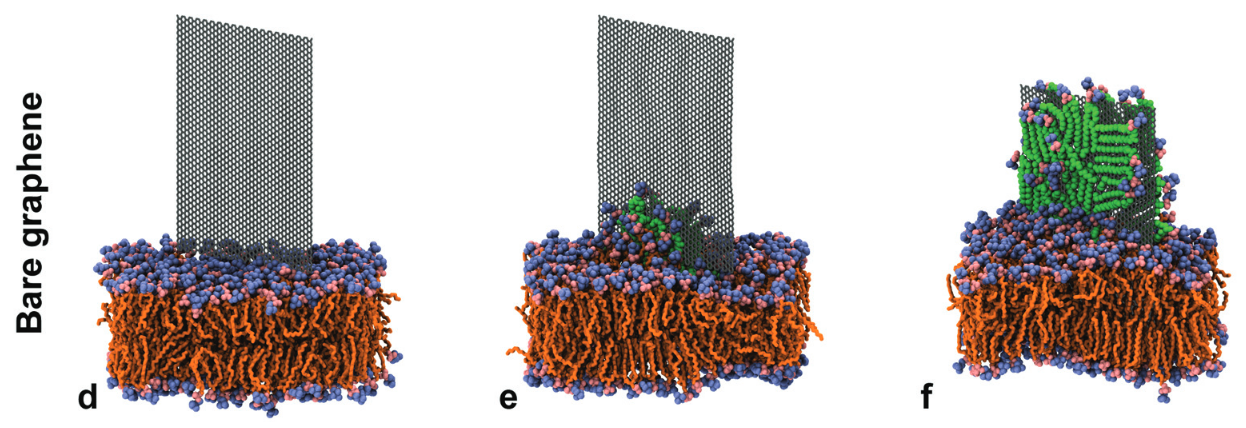
\includegraphics[width=.7\textwidth]{figures/Duan_2015a}
      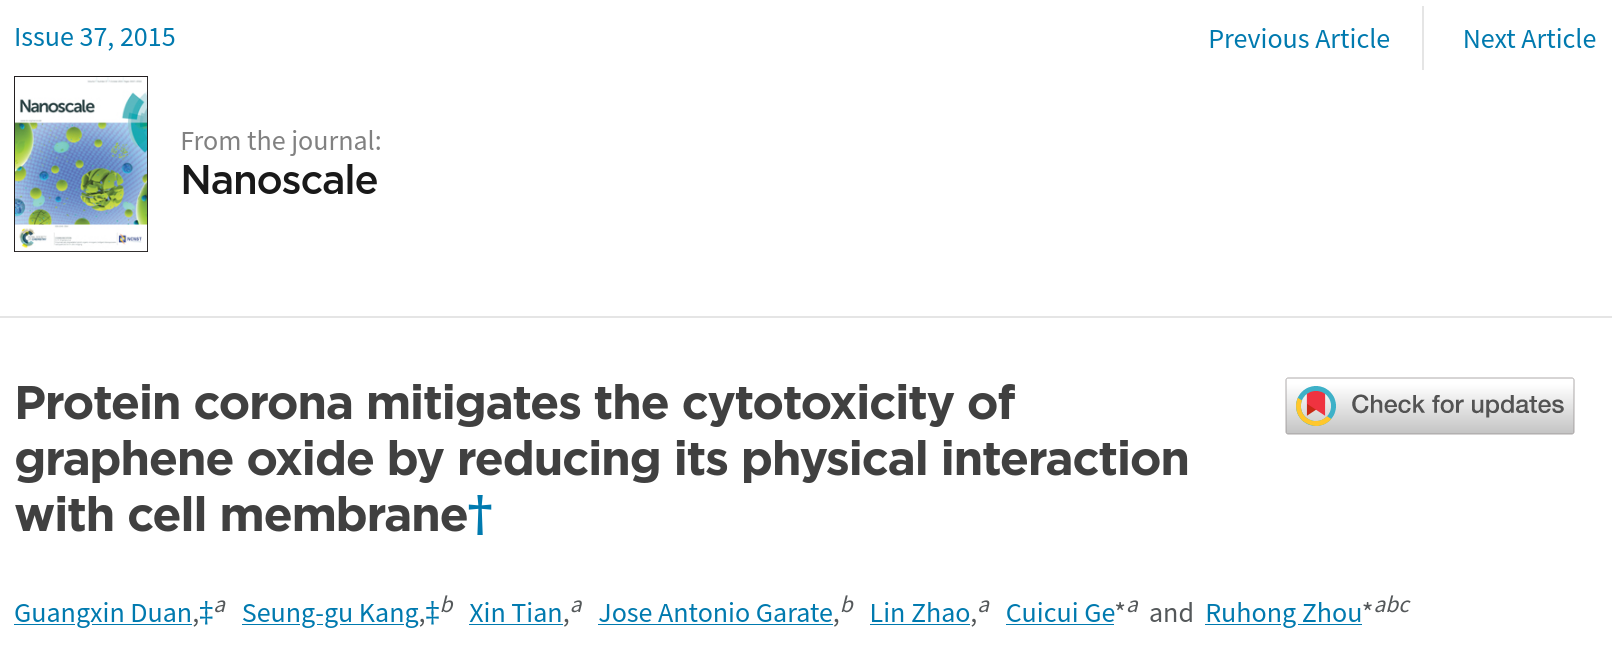
\includegraphics[width=.7\textwidth]{figures/Duan_2015}
\end{frame}


\begin{frame}

\begin{block}{However...}
\begin{itemize}
\item There is a lack of descriptions based on amino acid composition.
\item There is a lack of rigorous thermodynamic descriptions of
  adsorption processes on graphene.
\end{itemize}
\end{block}

\end{frame}

\begin{frame}{Simulations}
  \begin{columns}
    \begin{column}{.5\textwidth}
      \begin{block}{Free Energy of Adsorption}
        \begin{itemize}
        \item All proteinogenic amino acids are being studied.
        \item $\xi$ is defined as the distance between
          $\mathbf{q}_{\alpha-\mathrm{carbon}} $ and COM(graphene),
          times (dot product) $(0, 0, 1)$.
        \item $\Delta A_{ads} = A^{adsorbed} - A^{free}$
        \item $\Delta A_{ads}$ was calculated using GROMOS with
          the umbrella sampling method.
        \end{itemize}
      \end{block}
    \end{column}
    \begin{column}{.5\textwidth}
      \centering
      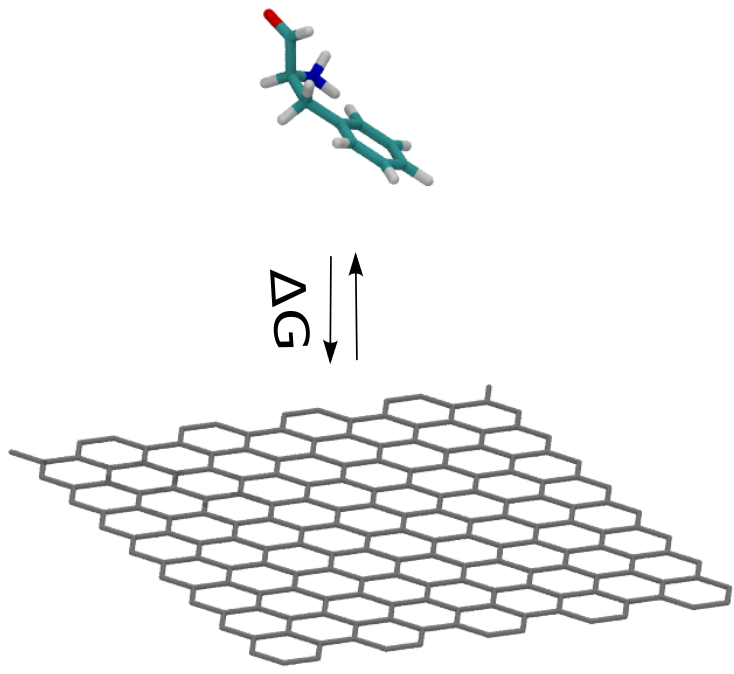
\includegraphics[width=\textwidth]{figures/Adsorption}
    \end{column}
  \end{columns}
\end{frame}

\begin{frame}{Simulated Systems}
  \begin{columns}
    \begin{column}{.5\textwidth} \centering
      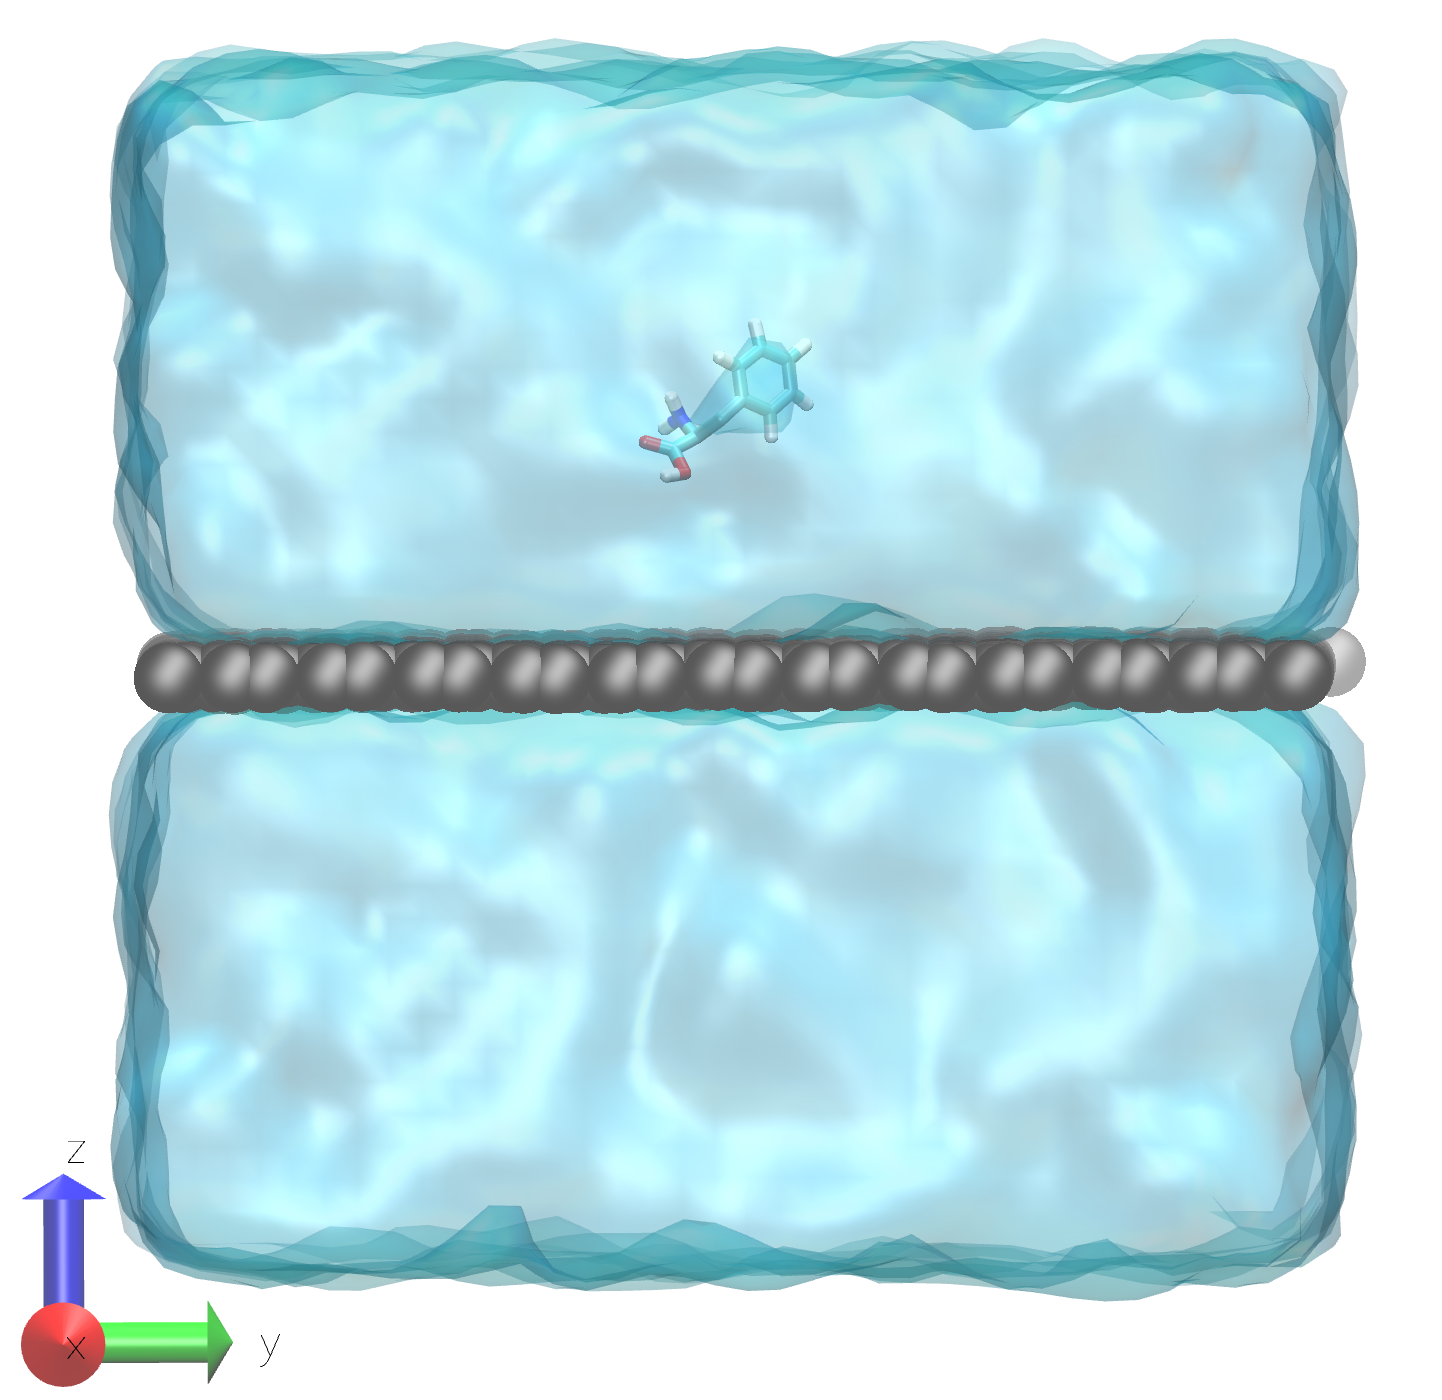
\includegraphics[width=.7\textwidth]{../../figures/Pristine_System.png}
    \end{column}
    \begin{column}{.5\textwidth}\centering
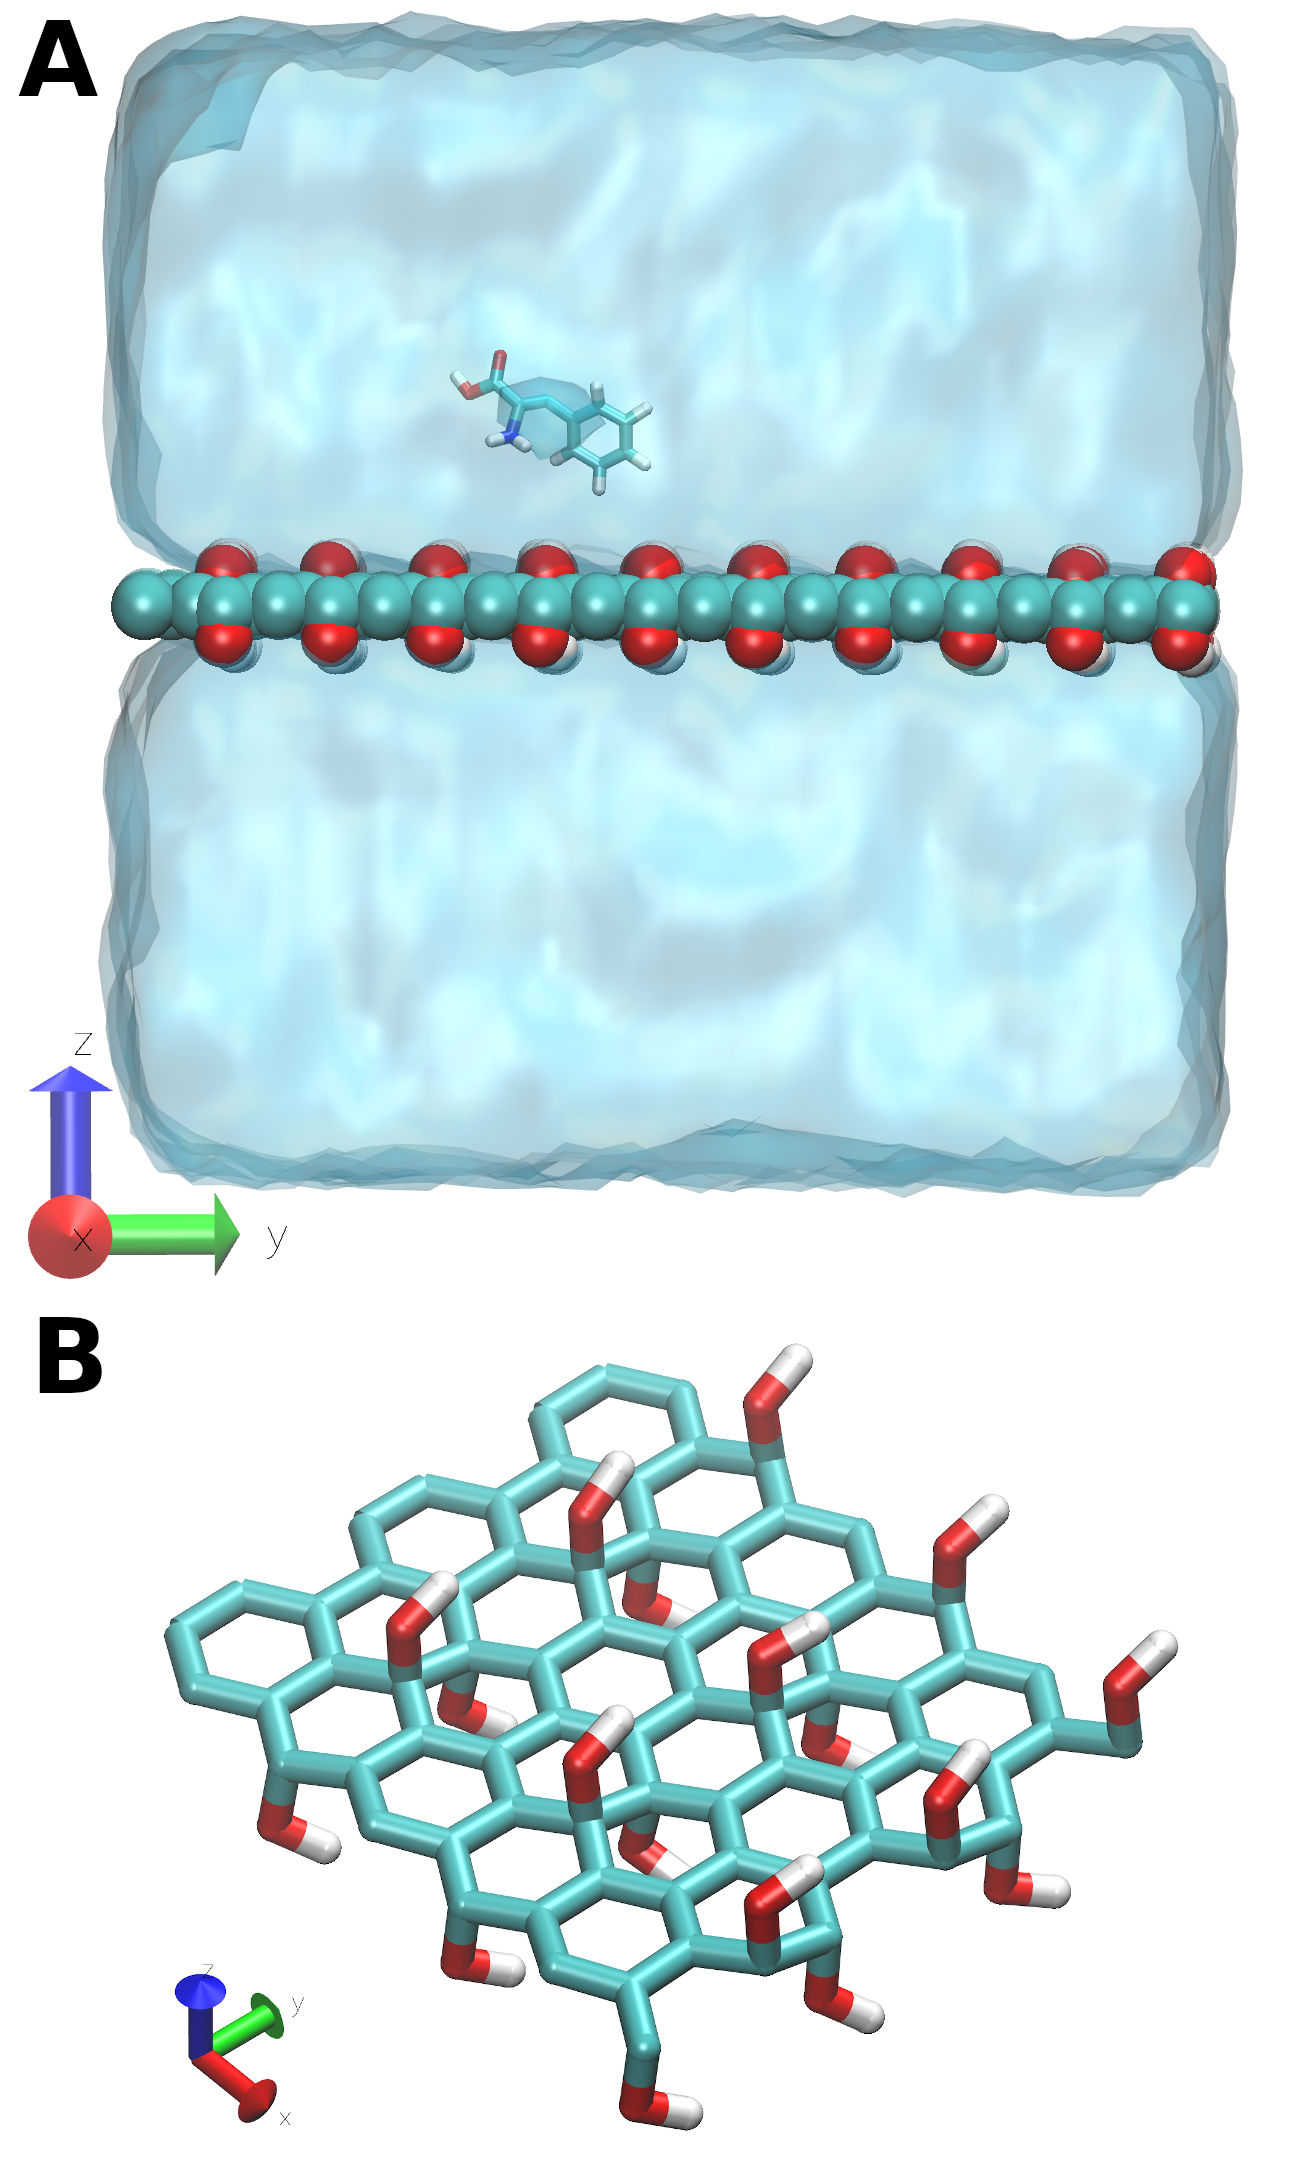
\includegraphics[width=.55\textwidth]{../../figures/Oxidized_System_and_Unit.png}
    \end{column}
  \end{columns}
\end{frame}

\begin{frame}{Free Energy, Energy, and Entropy}

\begin{columns}
\begin{column}{.5\textwidth}
\Large
  \begin{align*}
    \Delta A_{ads} &= \langle A \rangle_{adsorbed} - \langle A
    \rangle_{free} \\
    \langle A \rangle_{ab} &= \frac{\sum_{i=a}^b A(\xi_i)  p(\xi_i)
                             }{\sum_{i=a}^b p(\xi_i)} \\
    p(\xi_i) &= \frac{e^{-\beta \mathrm{PMF}(\xi_i)}}{\sum e^{-\beta \mathrm{PMF}(\xi)}}
  \end{align*}
\end{column}
\begin{column}{.5\textwidth}
  \Large
  \begin{align*}
    \Delta E_{ads} &= \langle E \rangle_{adsorbed} - \langle E
                     \rangle_{free} \\
    T\Delta S_{ads} &= \Delta E_{ads} - \Delta A_{ads}
  \end{align*}
\end{column}
\end{columns}
\end{frame}

\begin{frame}{Computing other properties}
\LARGE
  \begin{align*}
\langle T(\xi) \rangle = \frac{\sum_{i=1}^{M} \sum_{j=1}^{N_{i}} T_{i,
  j} e^{-\beta(A_i - V_{bias})} \delta \xi_{i, j}}{\sum_{i=1}^{M} \sum_{j=1}^{N_{i}} e^{-\beta(A_i - V_{bias})} \delta \xi_{i, j}}
\end{align*}
\end{frame}

\begin{frame}{$\Delta A^{ads}$, $\Delta E^{ads}$, $T \Delta S^{ads}$}
  \begin{columns}
    \begin{column}{.5\textwidth}
\centering
\resizebox{\linewidth}{!}{%
\csvreader[
  head to column names,
  before reading = \begin{center}\sisetup{table-number-alignment=center},
  tabular        = {lccc},
  table head     = \toprule \textbf{Amino acid} & $\Delta A$ & $\Delta E$ & $T \Delta S$ \\ \midrule,
  table foot     = \bottomrule,
  after reading  = \end{center},
  filter expr    = test{\ifnumless{\thecsvinputline}{15}}
  ]{/home/mbarria/Dropbox/Papers/graphene_adsorption_paper/data/tables/Free_Energy_Decomposition.csv}{3=\Aerr, 5=\Eerr, 7=\Serr}{%
   \Name & \myround\dA~$\pm$\myround\Aerr & \myround\dE~$\pm$\myround\Eerr & \myround\TdS$~\pm$\myround\Serr %&
}
 }
    \end{column}
    \begin{column}{.5\textwidth}
\centering
\resizebox{\linewidth}{!}{%
\csvreader[
  head to column names,
  before reading = \begin{center}\sisetup{table-number-alignment=center},
  tabular        = {lccc},
  table head     = \toprule \textbf{Amino acid} & $\Delta A$ & $\Delta E$ & $T \Delta S$ \\ \midrule,
  table foot     = \bottomrule,
  after reading  = \end{center},
  filter expr    = test{\ifnumgreater{\thecsvinputline}{14}}
  ]{/home/mbarria/Dropbox/Papers/graphene_adsorption_paper/data/tables/Free_Energy_Decomposition.csv}{3=\Aerr, 5=\Eerr, 7=\Serr}{%
   \Name & \myround\dA~$\pm$\myround\Aerr & \myround\dE~$\pm$\myround\Eerr & \myround\TdS$~\pm$\myround\Serr %&
}
 }
    \end{column}
  \end{columns}
\end{frame}



\begin{frame}{Adsorption over Pristine Graphene}
\centerline{\includegraphics[width=1\textwidth]{/home/mbarria/Dropbox/Papers/graphene_adsorption_paper/figures/Differences_by_names_and_weight.png}}
\end{frame}

\begin{frame}
\centering
\resizebox{\linewidth}{!}{%
\csvreader[
  head to column names,
  before reading = \begin{center}\sisetup{table-number-alignment=center},
  tabular        = {lccc},
  table head     = \toprule \textbf{Amino acid} & $\Delta A$ & $\Delta E$ & $T \Delta S$ \\ \midrule,
  table foot     = \bottomrule,
  after reading  = \end{center},
  ]{/home/mbarria/Dropbox/Papers/graphene_adsorption_paper/data/tables/Free_Energy_Decomposition_25o.csv}{3=\Aerr, 5=\Eerr, 7=\Serr}{%
   \Name & \myround\dA~$\pm$\myround\Aerr & \myround\dE~$\pm$\myround\Eerr & \myround\TdS$~\pm$\myround\Serr %&
}
 }
\end{frame}



\begin{frame}{Adsorption over Oxidized Graphene}
\centerline{\includegraphics[width=1\textwidth]{/home/mbarria/Dropbox/Papers/graphene_adsorption_paper/figures/Differences_by_names_and_weight_25o.png}}
\end{frame}

\begin{frame}{Adsorption of Penta-Alanine over pristine graphene}
\centering
\begin{tabular}{lccc}
\toprule
Alanine & $\Delta A^{ads}$ & $\Delta E^{ads}$ & $T \Delta S^{ads}$ \\
Mono & $ -10.3 \pm 0.1 $ & $ -12.5 \pm 1.8 $ & $ -2.2 \pm 1.8 $ \\
Penta (Prediction) & $ -43.3 \pm 0.4 $ & $ -52.5 \pm 7.6 $ & $ -9.24 \pm 7.6$ \\
Penta (Stretched) & $ -40.4 \pm 0.1 $ & $ -48.8 \pm 6.7 $ & $ -8.4 \pm 6.7 $ \\
Penta (Helix) & $ -6.3 \pm 0.1 $ & $ -32.6 \pm 5.4 $ & $ -26.2 \pm 5.5 $ \\
\bottomrule
\end{tabular}
\end{frame}


\end{document}

%%% Local Variables:
%%% mode: latex
%%% TeX-master: t
%%% End:
